This chapter shows how to apply the control method presented in Chapter \ref{chap_SDNNetSim} to a real network with dedicated hardware. Subsequently, it is tested how it is possible to obtain excellent traffic predictions on a network device of an italian internet provider (Sonicatel s.r.l.).
\section{Control performance validation over dedicated hardware network}
Given the limitations of the Mininet software, it has been decided to test the previously explained algorithms on a real network. Due the fact that the SDN network devices are much expensive, it has been choosen to take an intermediate step in which each device is associated with a dedicated hardware, unlike Mininet in which multiple virtual devices shared single hardware resorces. The used architecture is shown in Figure \ref{fig:{Real_NET}}, where two Raspberry pi 3 \cite{rasp} has been used has hosts connected on a single switch. Moreover the SDN switch resides in a third Raspberry, where the firmware of an OVS has been installed and two ethernet/usb adapter has been used as ethernet ports (eth1 and eth2) to connect the hosts. The built in ethernet port (eth0) has been used to connect the SDN controller (RYU) to the switch. An Arduino UNO with a DS1307 module has been used to share single time schedule from the controller to the hosts. By using the python script in \ref{ReadTime}  it has been possible to iteratively update the time on DS1307 module every hour, then each raspberry can update its internal time by asking the time to module via $I^{2}C$ serial communication. Every update is performed in different minute of the same hour to avoid collisions caused by multiple requests. This time sharing has been necessary to ensure time synchronization between traffic generation and data harvesting. In a real network the time synchronization is ensure to internet time sharing.
\begin{figure}[tb!]
	\centering
	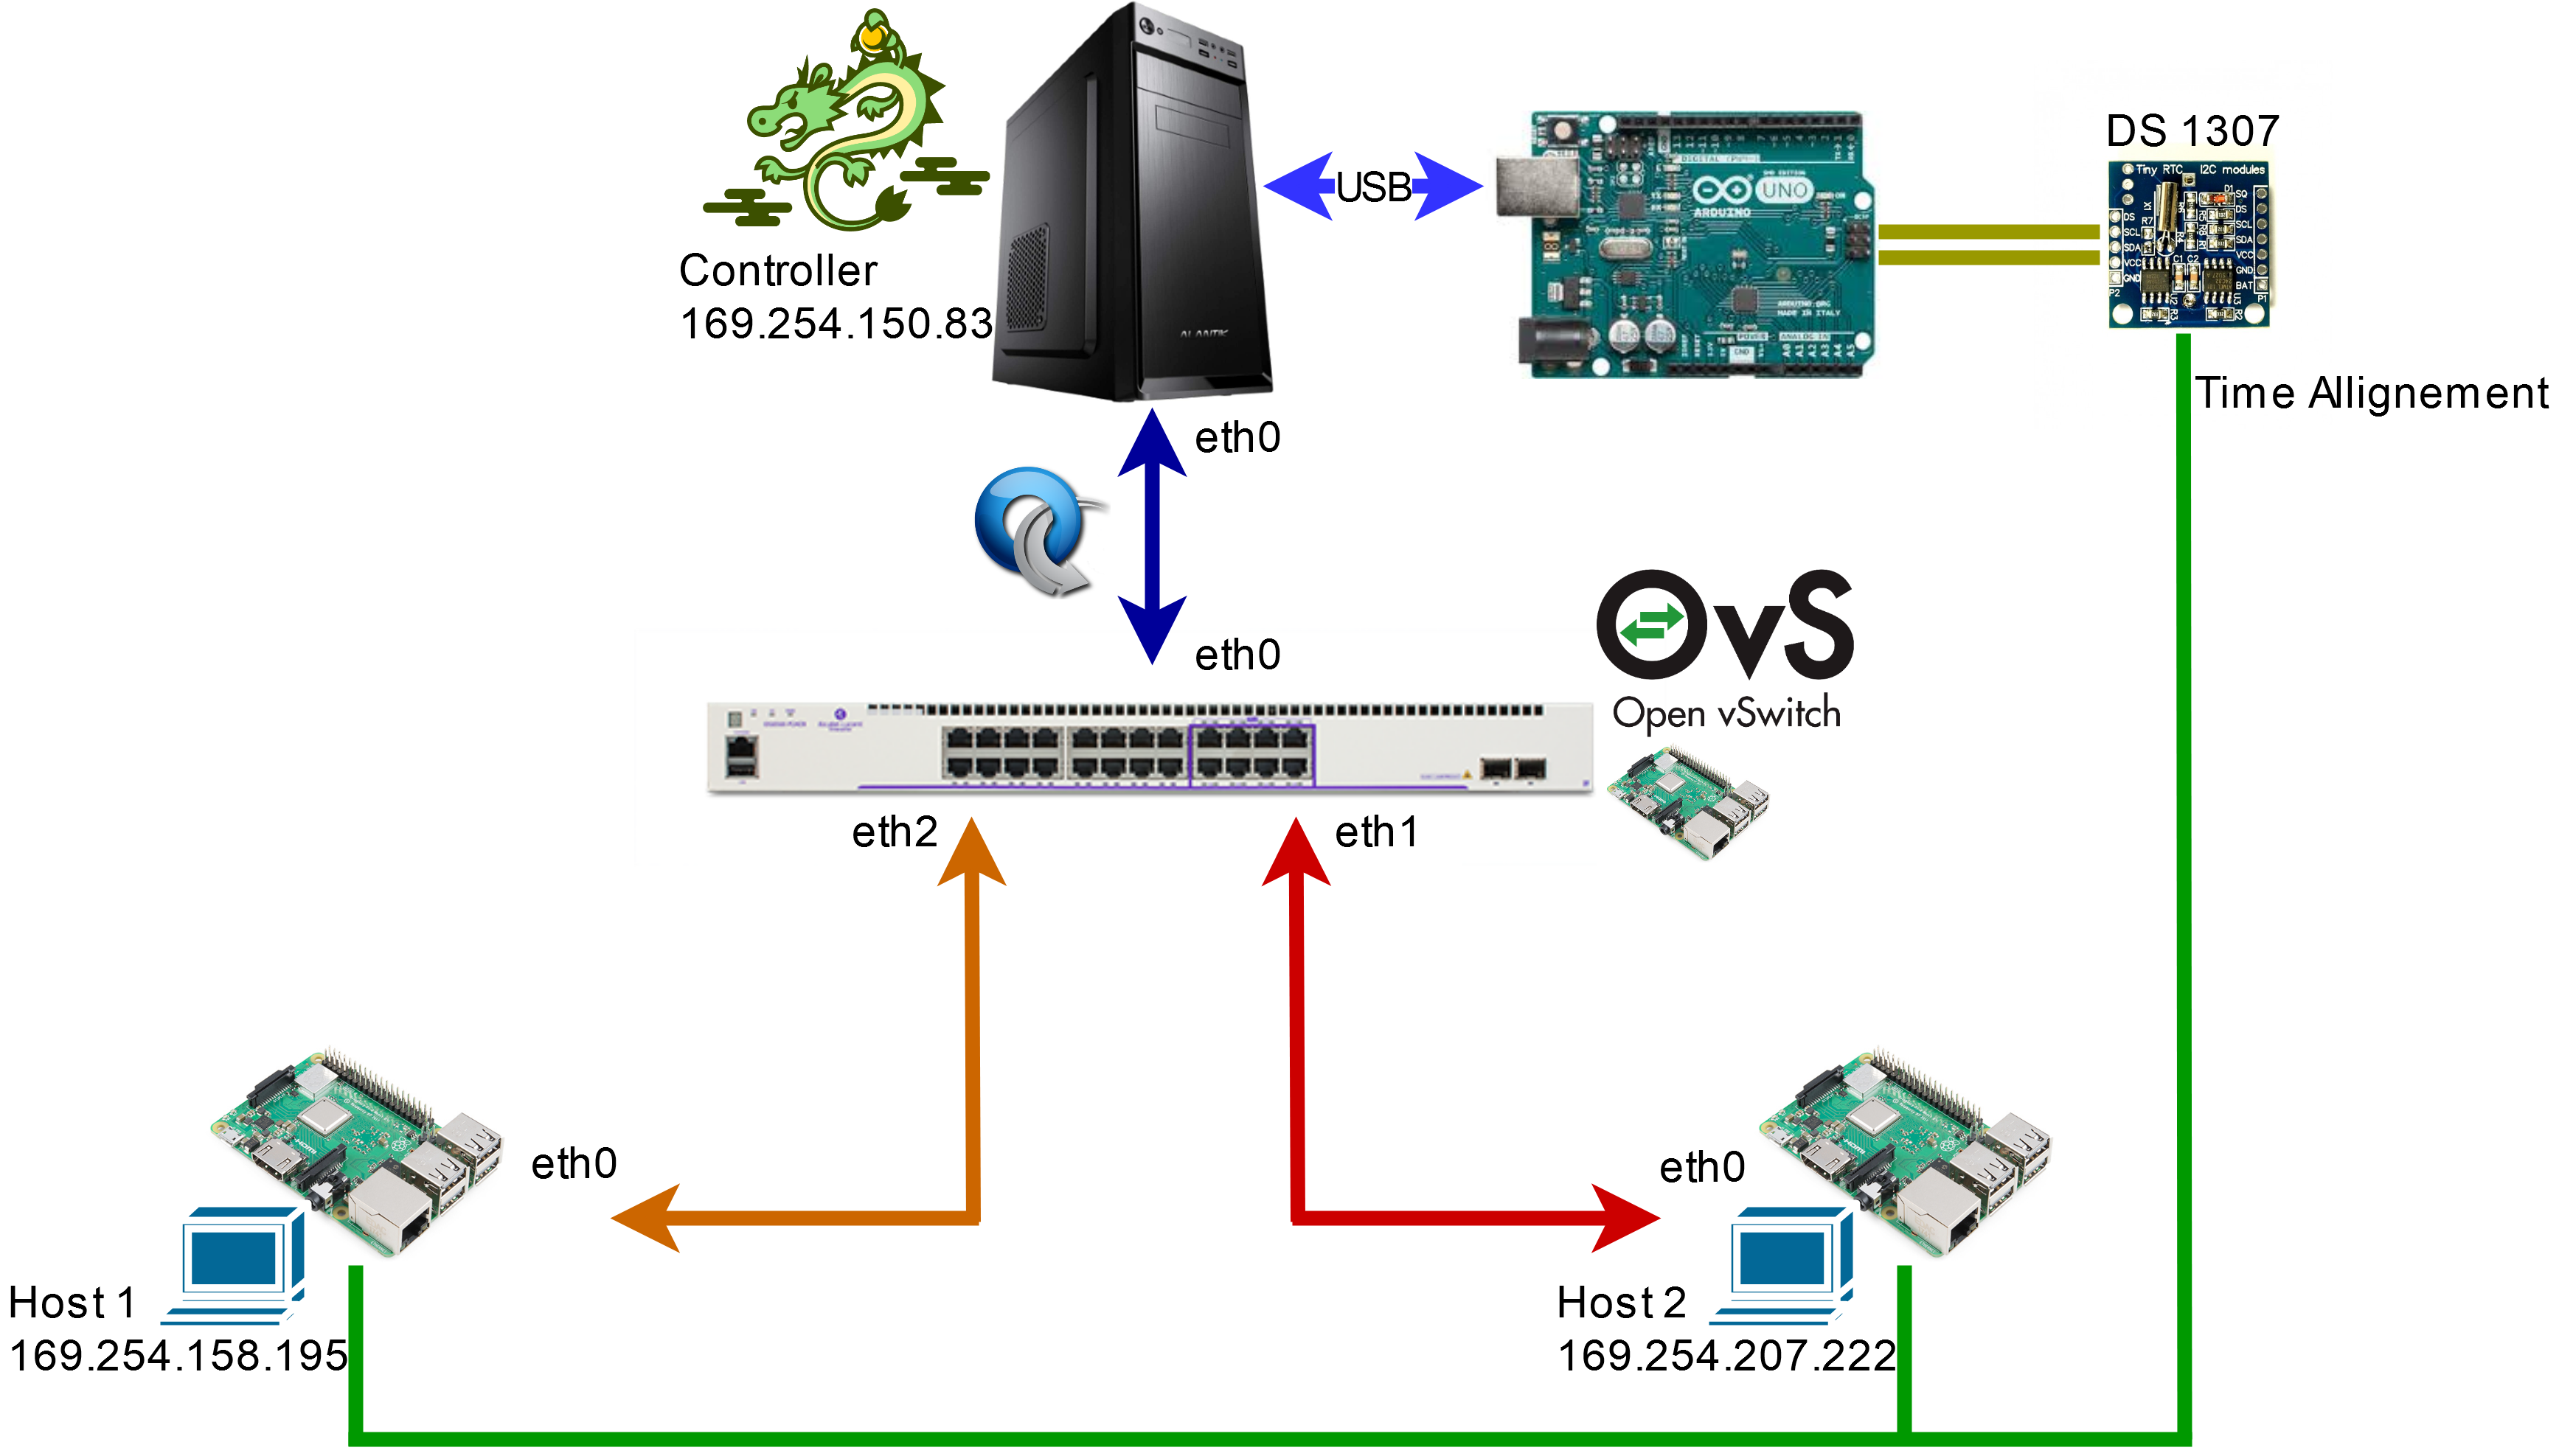
\includegraphics[width=13cm]{figure/Real_NET.png}
	\caption{Network architecture with dedicated hardware devices.}
	\label{fig:{Real_NET}}
\end{figure}
Even in this environment Ryu controller has been used as SDN controller with the same Python script previously described for Mininet network (e.g. \ref{datapath_monitor_TOS}, \ref{main_controller_TOS} and \ref{Controller_commands}). The custom flow table rules are set after the deploy of the controller and after the join of the switch by a single run of the code in \ref{Set_Queue}. With this operation we have the default set up has in section \ref{sec:SDNNetSim} (e.g. three queues on port 2 with a bandwidth of $100Mbps$ and 20\% of port bandwidth for queue 0, 80\% of port bandwidth for queue 1 and 100\% of port bandwidth for queue 2). While for Mininet emulator we had a single code in which both the network topology and the traffic generation of each host were present (e.g. \ref{Topology}), in the case of dedicated hardware it was necessary to write a new Python script that included the generation and reception of traffic and infinitely run it on the two Raspberry that act as hosts. The code \ref{Traffic_Real_Hwd} contain two different thread: the first one is very similar to the part of code contained in \ref{Topology} for the generation of the traffic, the only difference is the IP address of the hosts. The second thread is very simple and is needed to start the DITG Receiver module on each host. After some tests it has been possible to see that in the hours where there are the highest number of packets incoming in the switch the computational capacity of a Raspberry pi 3 is not sufficient to elaborate all the necessary operations to route the packets to the hosts. Thus it has been decided to send packets only from $Host 2$, with IP address $169.254.207.222$, to $Host 1$, with IP address $169.254.158.195$. With this traffic generation no anomaly was found on the information obtained from the OF counters as showed in Figure \ref{fig:PKTS_REAL}(a). This figure shows packets coming into the switch generated by $Host 2$ (blue line) and packets outgoing from port 2 of the switch to $Host 1$ (red line), in case the MPC control policies explained in Section \ref{secSwitchedModeling} are applied with the same mathematical model used in Section \ref{sec:control_performance}. This figure makes it clear that the traffic generation is different than the traffic generated by virtual hosts in Mininet. In particular, in the last hours of the day there is a much higher traffic peak than emulation, how showed in Figure \ref{fig:PKTS_REAL}(b). This is probably caused by sharing multiple network devices on a single hardware that decrease the performance of each network element. With this traffic generation difference is difficult to compare the results come from those environment. Due the chosen limitation of the queues bandwidth it has been possible to see in Figure \ref{fig:PKTS_REAL}(c) that the amount of packets transmitted from the controlled port it's about the same between the two network setups, even after one model update like the one explained in Section \ref{secExpRes}. This last very important result demonstrates how it is possible to use a virtual network to train a mathematical model aimed to controlling some device features and then apply this controller to a likely real network while maintaining the same traffic profile. Furthermore, another interesting aspect that emerges from these data is that even after an update of the control model, therefore after adding a traffic profile different from the one already present, the overall behavior of the queues remains practically unchanged. This set of results paves the way for experimentation on real networks.
\begin{figure}[H]
\centering
\subfigure[a][]{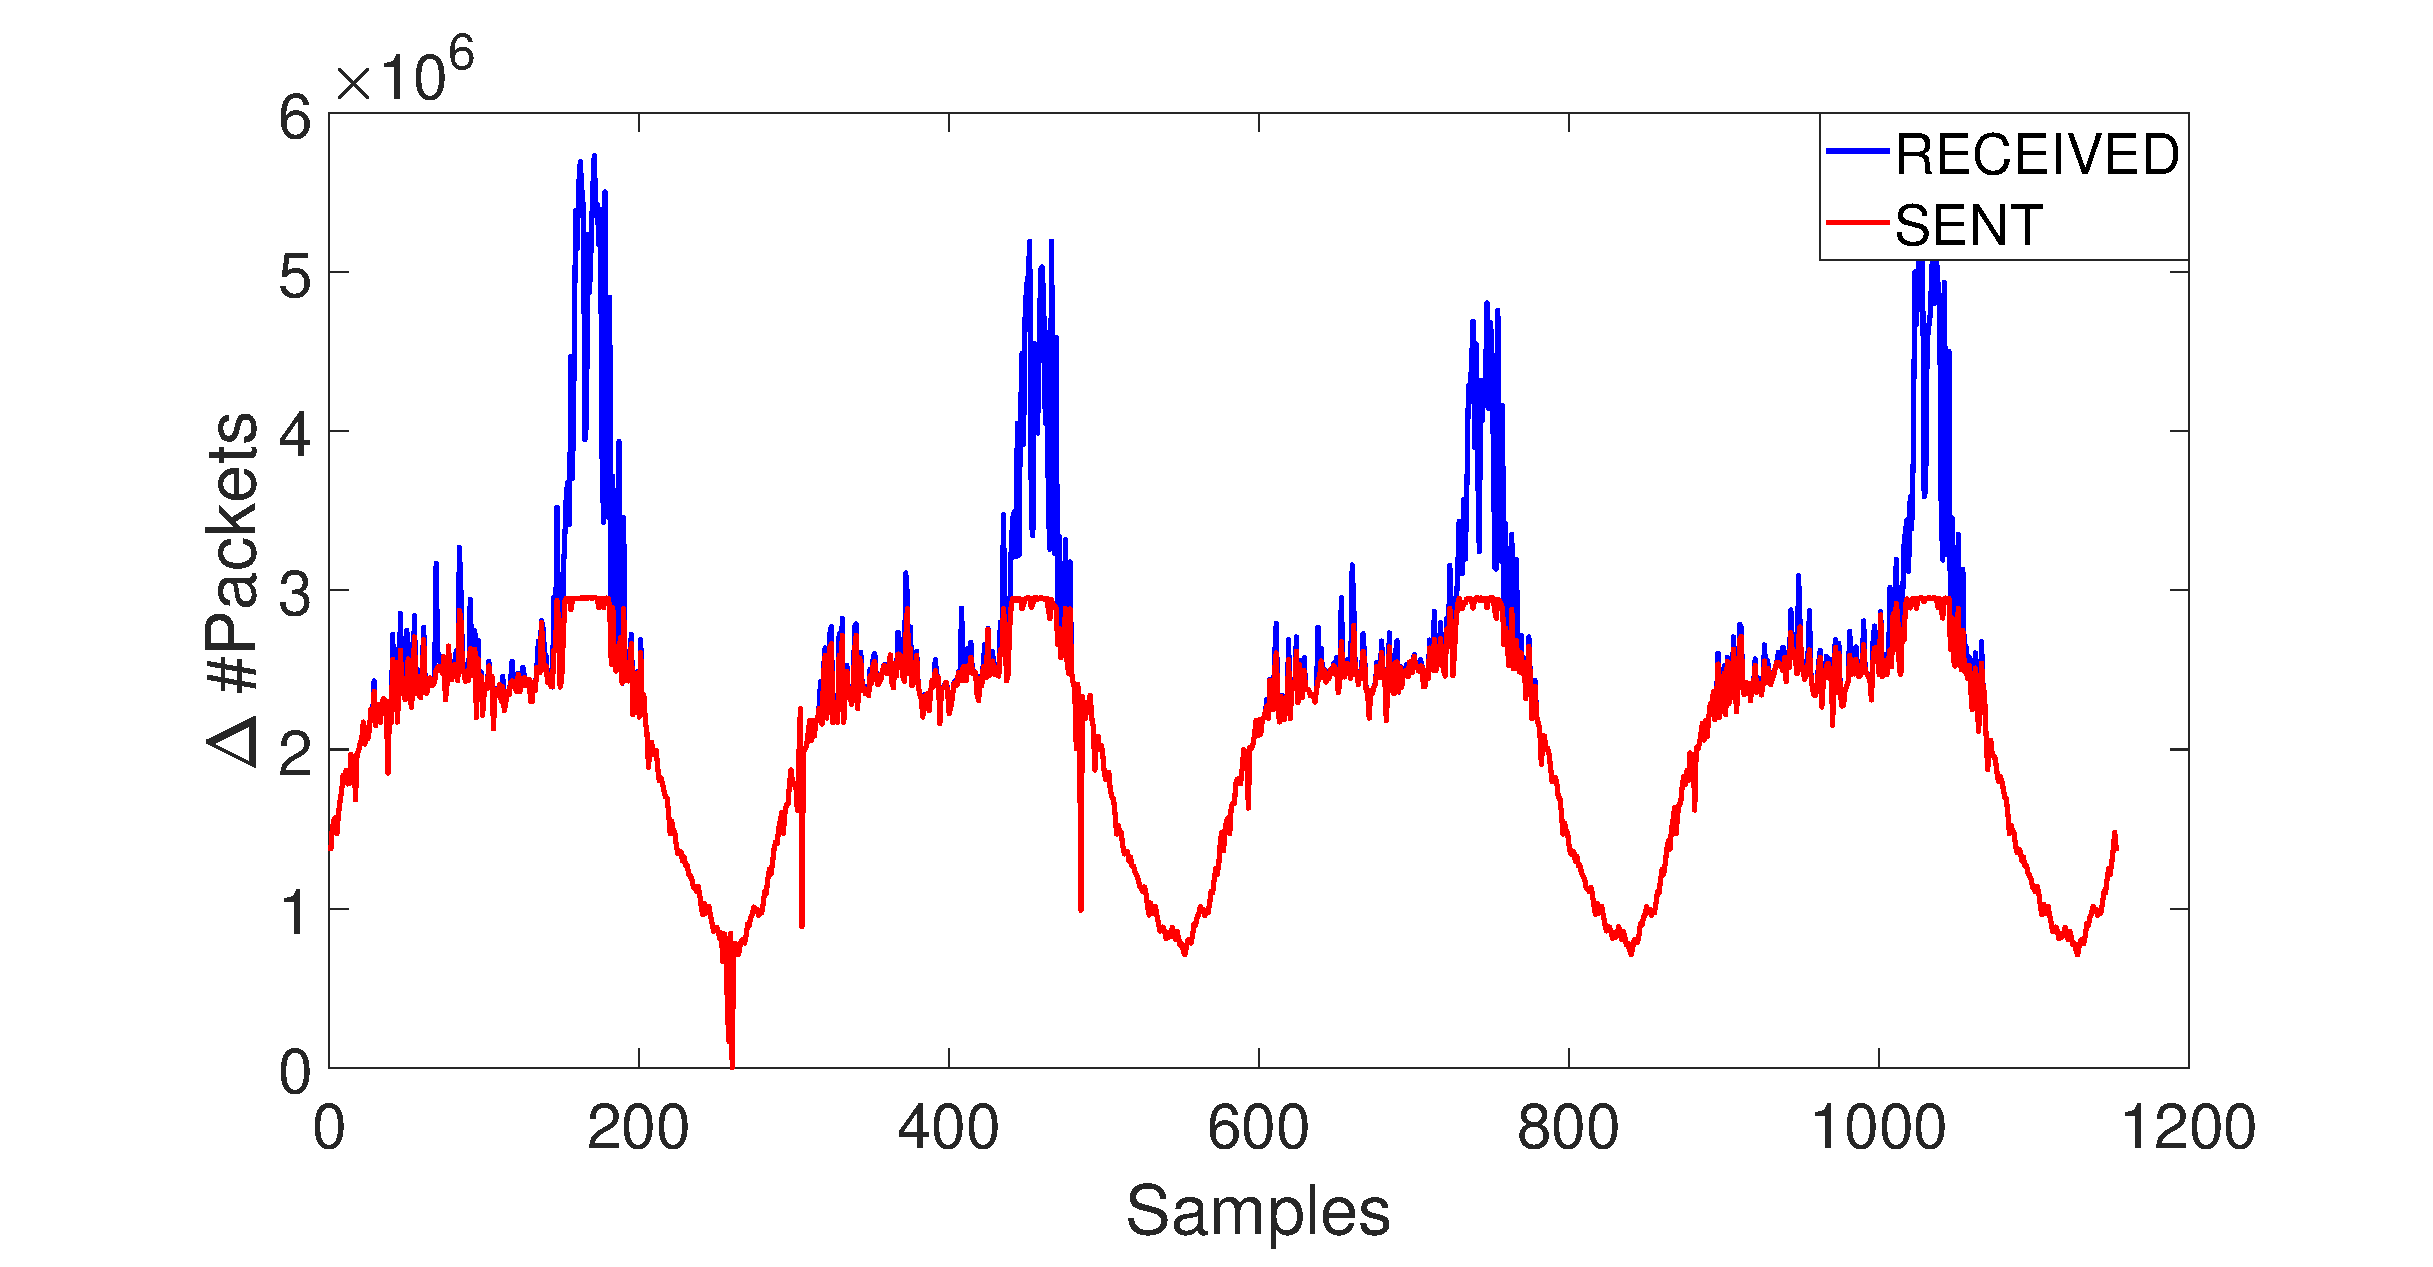
\includegraphics[width=0.7\linewidth]{figure_Real_HW/PKTS_RX_TX_realHWD.eps}}
\subfigure[b][]{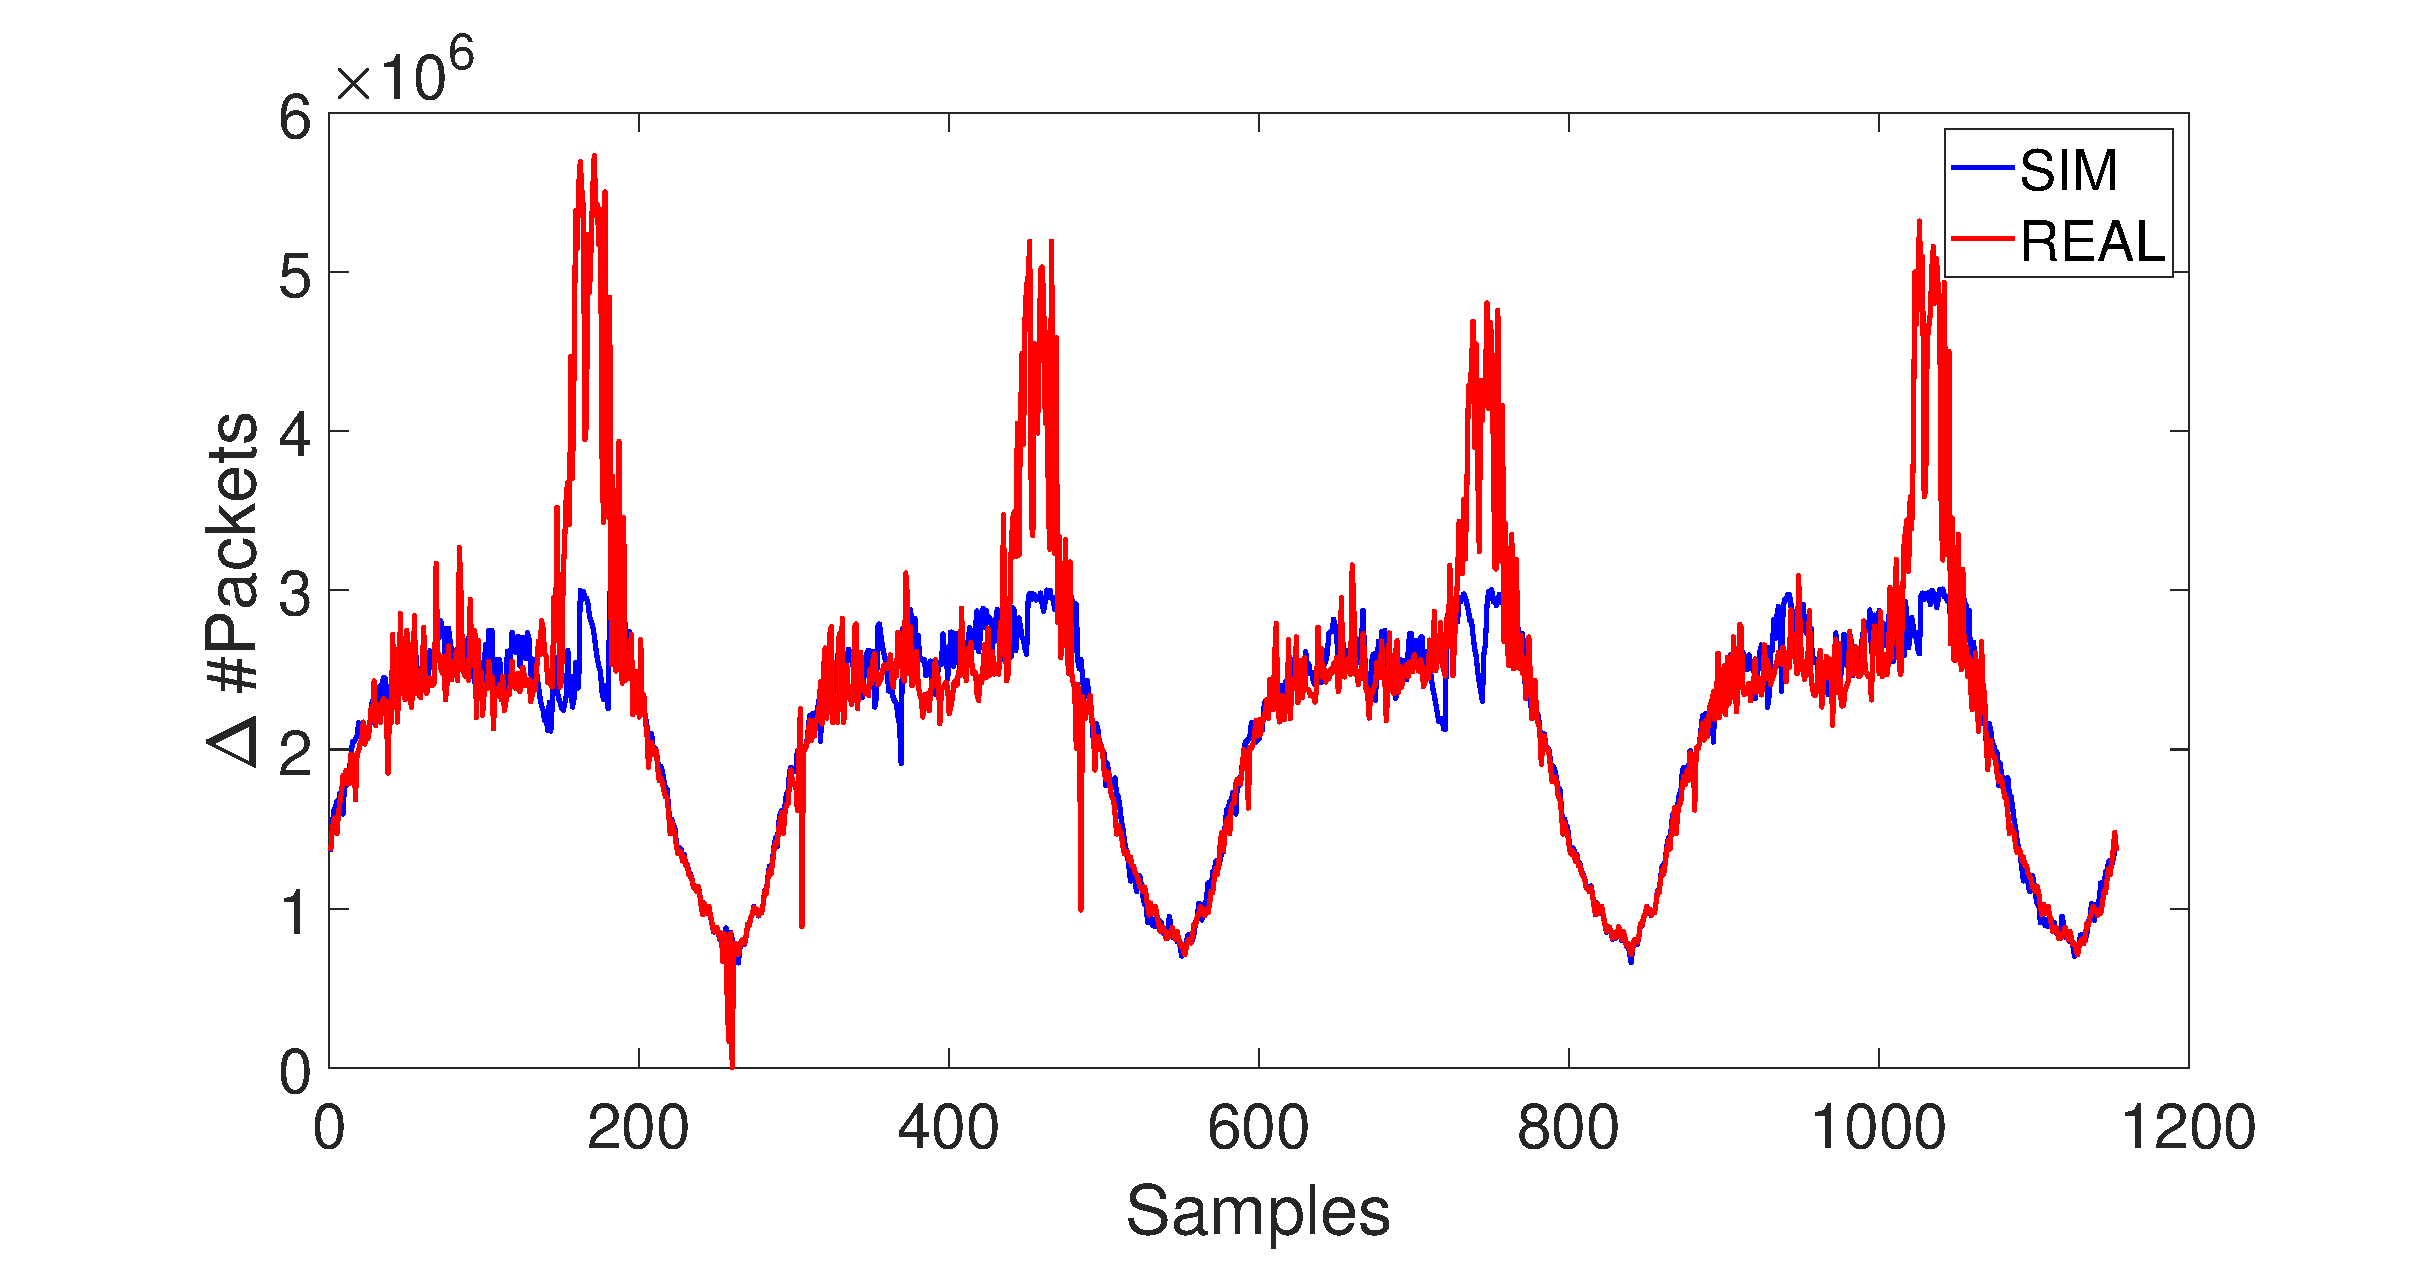
\includegraphics[width=0.7\linewidth]{figure_Real_HW/PKTS_RX.eps}}
\subfigure[c][]{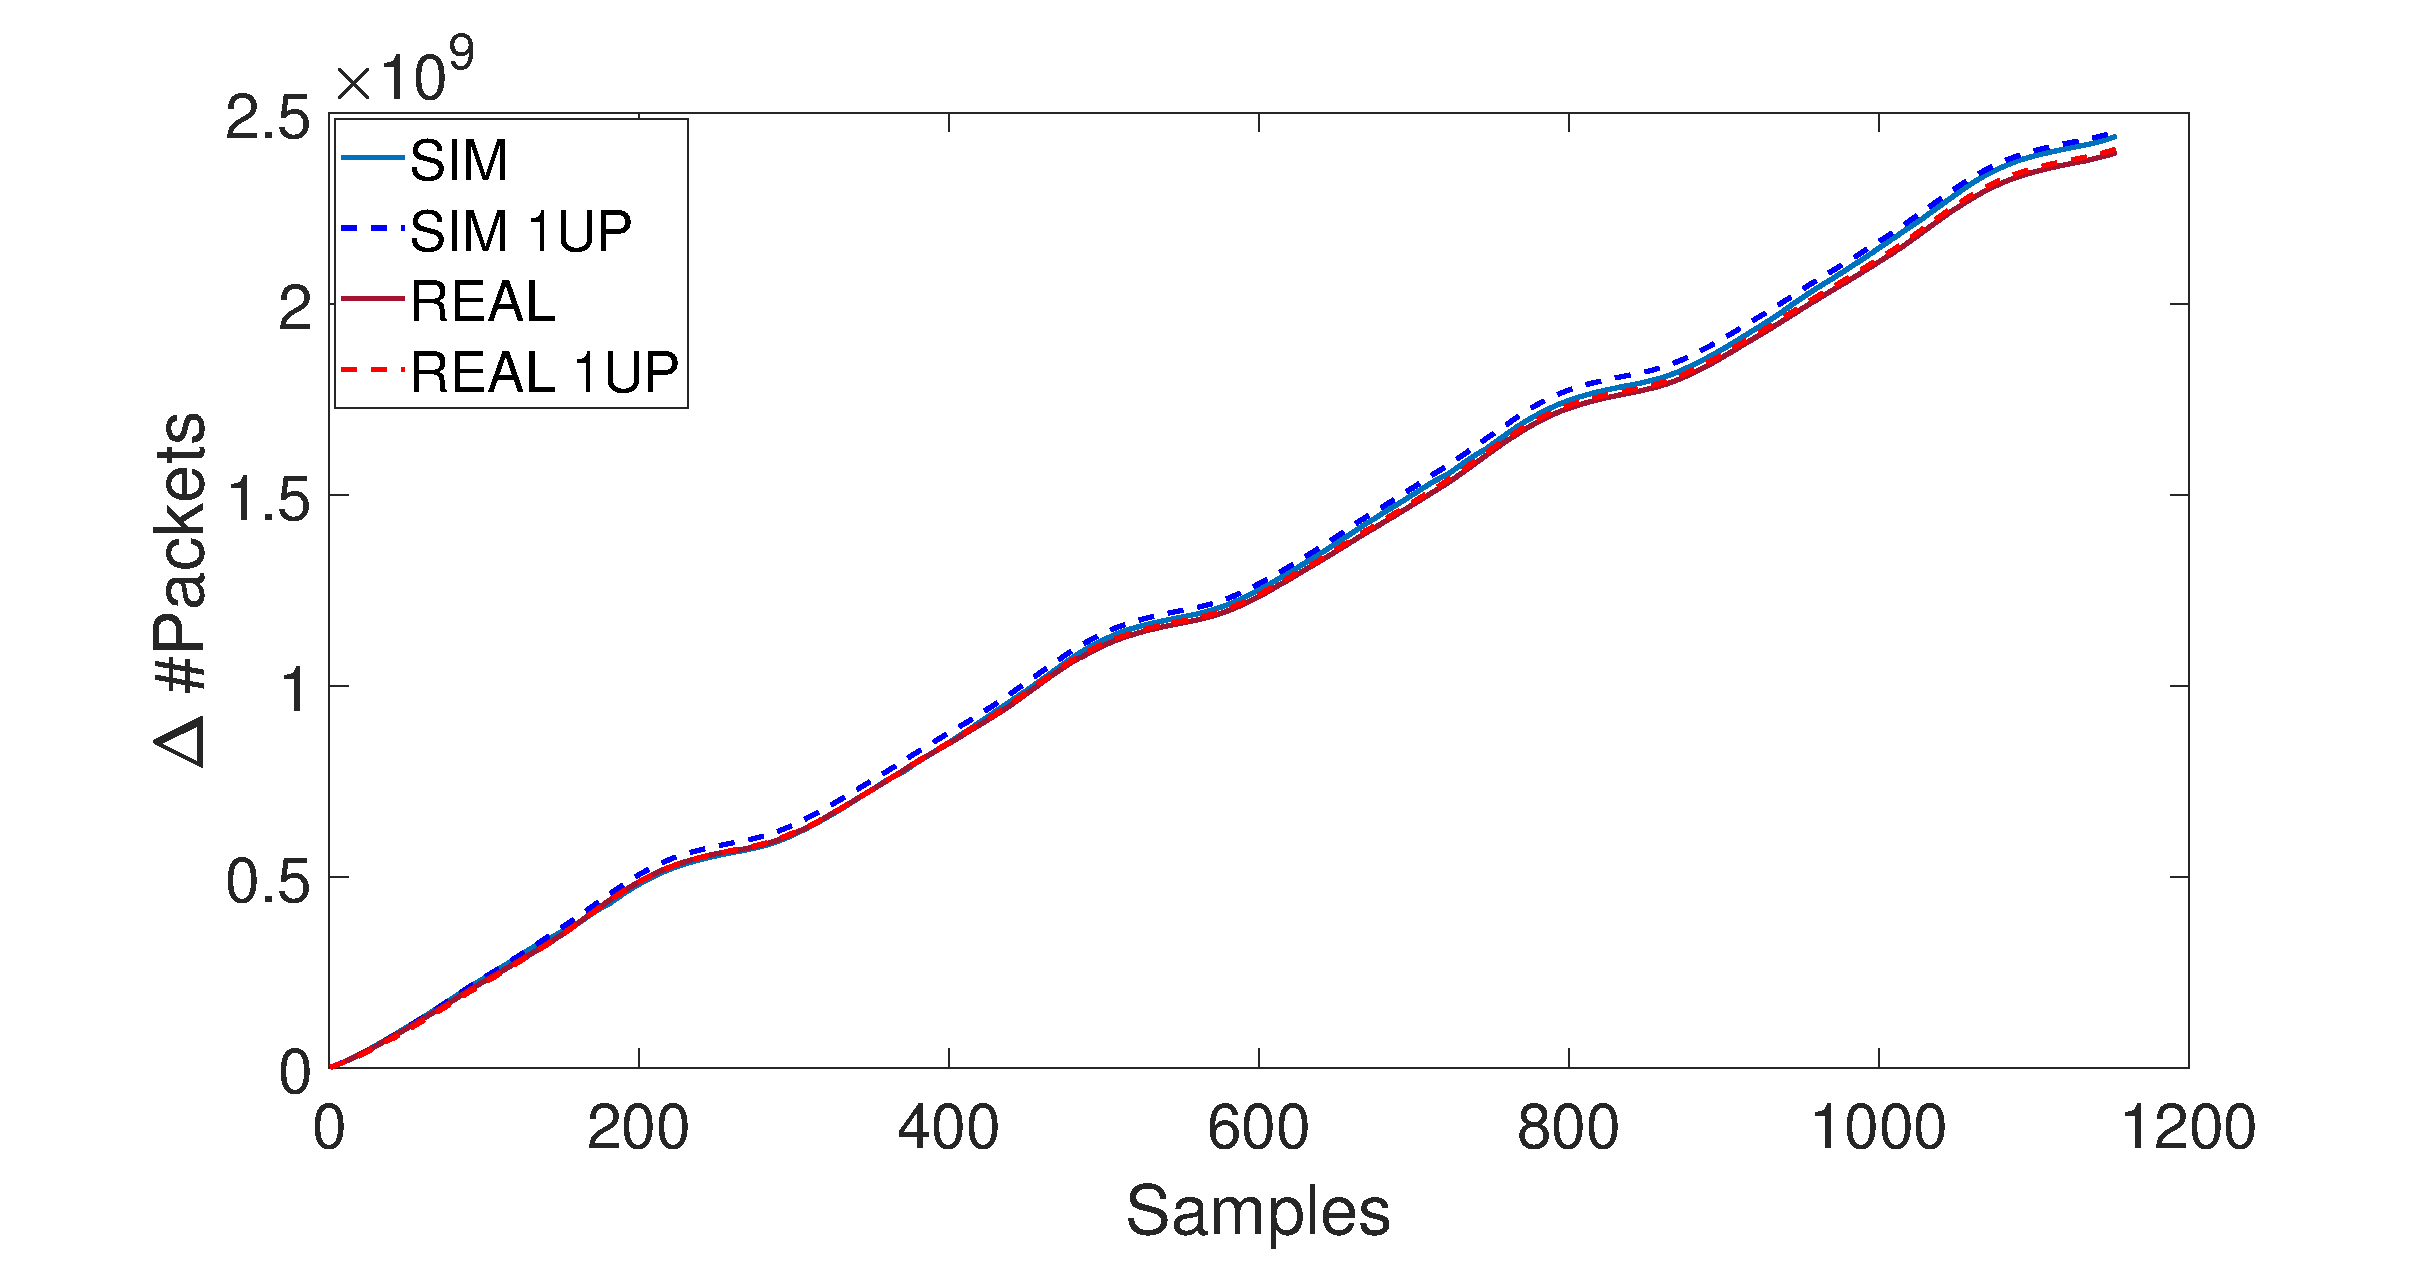
\includegraphics[width=0.7\linewidth]{figure_Real_HW/SUM_TX.eps}}
\caption{Packets that transit inside the switch (a), comparison between packets incoming in the switch in emulation environment and in dedicated hardware (b) and sum of packets sent by the switch port with different control model (c).}
\label{fig:PKTS_REAL}
\end{figure}
\
\section{Traffic predictive model validation on Italian Internet provider network}
In addition to the validation of our predictive models of the incoming traffic over the Mininet environment and dedicated hardware devices network, the accuracy has been also tested on data measured from a real network device (Ubiquiti EP-16) of an Italian internet provider (Sonicatel S.r.l.). Data collection has been performed using the software Cacti \cite{Cacti}.\\
\begin{figure}[H]
	\centering
	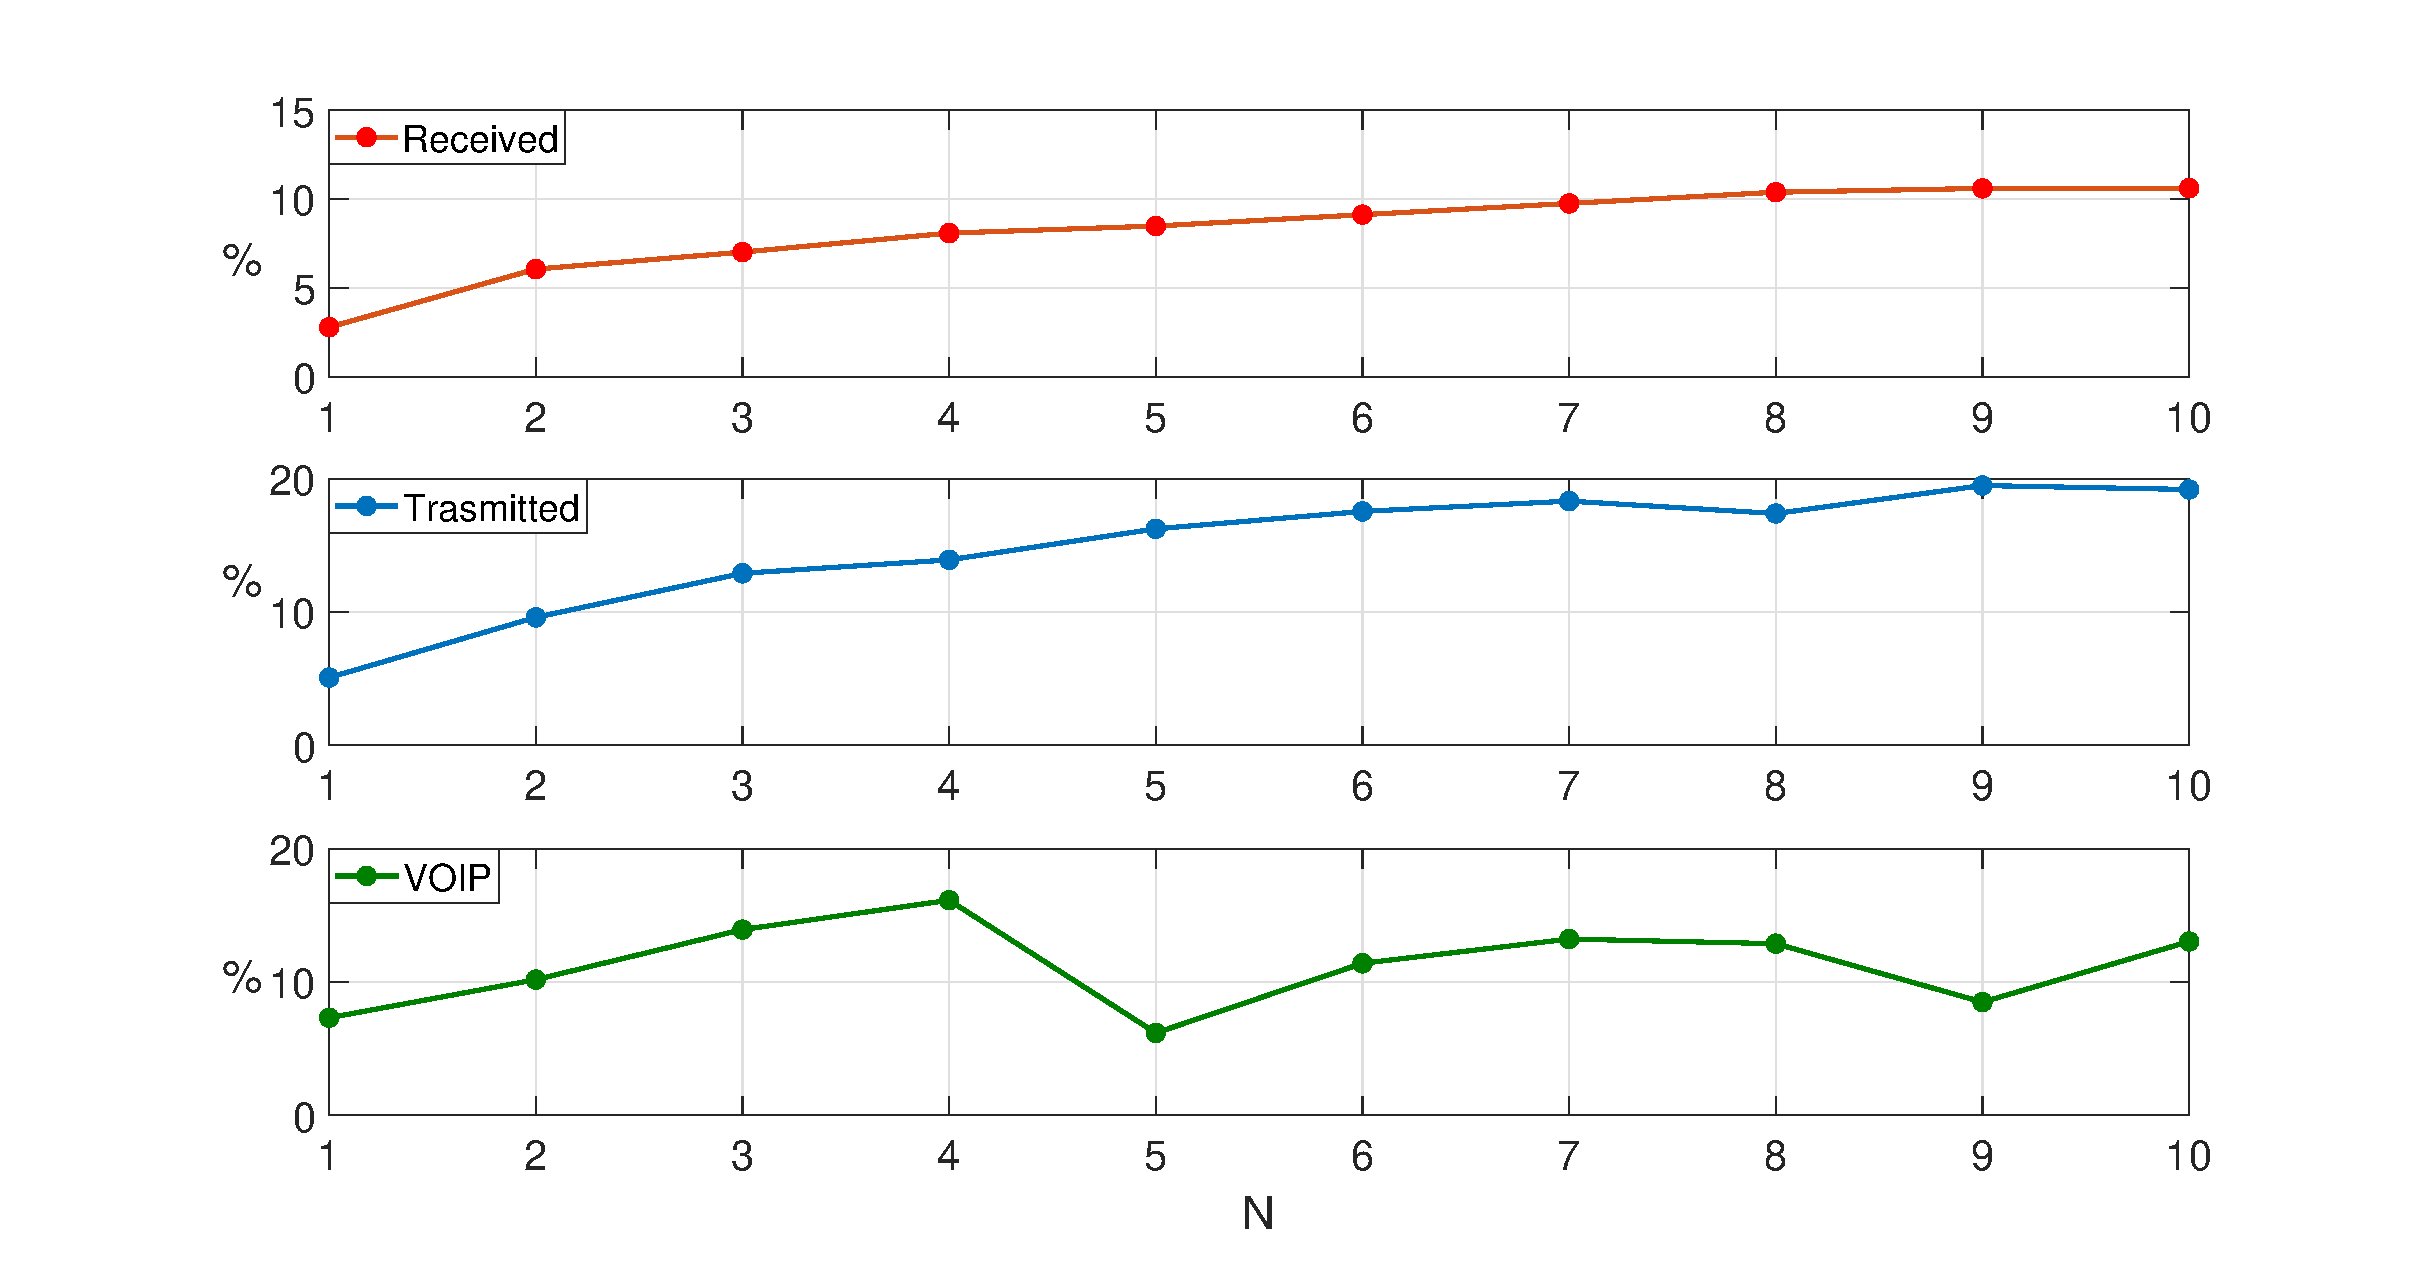
\includegraphics[trim={120 0 120 0}, width=1\linewidth]{figure/Error_PESCARA_DATA.eps}
	\caption{NRMSE of the packets predictive model over a time horizon of $N=10$.}
	\label{fig:{errorPescara}}
\end{figure}
Since this device is part of a running commercial network, some constraints in data collection have forced to only measure the sum of all packets entering and leaving the device, and it has been possible to extract from such traffic only incoming VOIP packets: i.e., it has not been possible to extract packets differentiated for each DSCP. Moreover, it is not currently possible to apply any type of closed-loop control on the network device. For the above 2 reasons the control performance has not been validated.\\
About data analysis, 53 days of data measurements have been used for RF training and about 3 days for model validation. Figure \ref{fig:{errorPescara}} shows the prediction on three classes of packets: all packets received, all packets transmitted, VOIP packets received. The plots show that our methodology provides a very accurate prediction even on a real internet service provider network.\\
After few months it has been possible to extend our trained model, using a total of $26138$ samples, with the same method previously explained in section \ref{secExpRes}. This model has been validated on a test of $19144$ samples, i.e. on more than two months of measurements. Even though the test pool is so large, thanks to the variety of train data it has been possible to obtain very low error values on packet prediction, as shown in Figure \ref{fig:{LONGTEST_Pescara}}.
\begin{figure}[H]
	\centering
	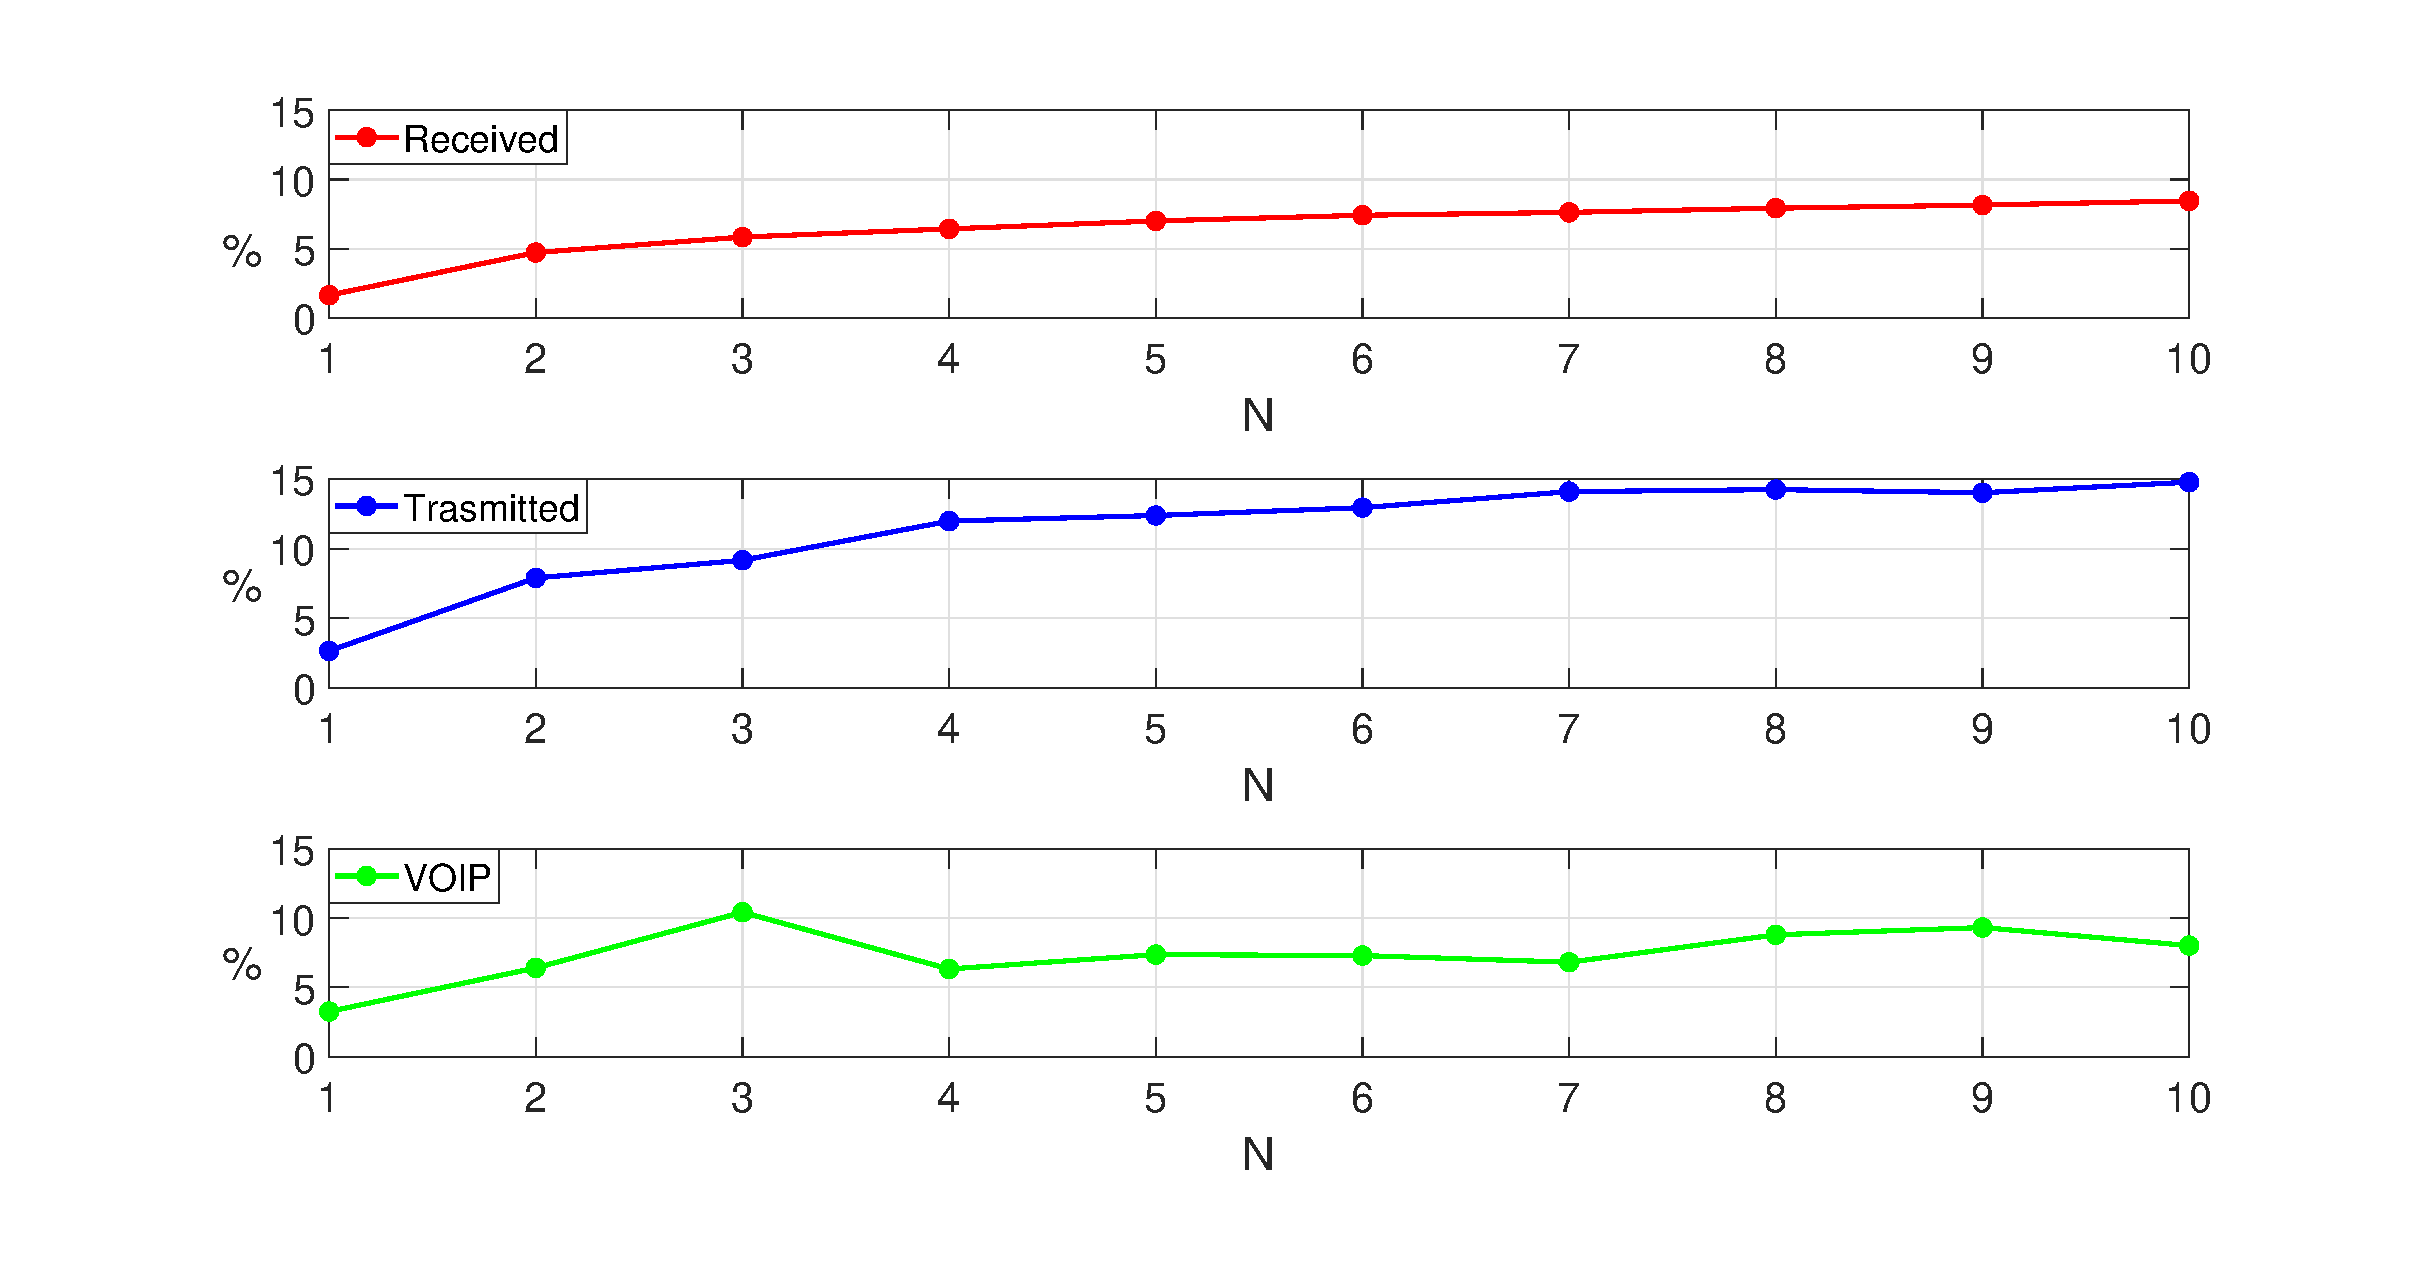
\includegraphics[trim={120 0 120 0}, width=1\linewidth]{figure/LONGTEST_PESCARA.eps}
	\caption{NRMSE of the packets predictive model over a time horizon of $N=10$ after one data update.}
	\label{fig:{LONGTEST_Pescara}}
\end{figure}
At a later time Sonicatel S.r.l. needed to move the monitored device to another location on their network by connecting different users with different contracts and therefore with different traffic profiles. This has been a great opportunity to validate the proposed method as it has been possible to test the network device computed model with a traffic pattern totally unrelated to the training data-set. This test could lead to two conclusions:\\
1) The prediction error could have been too high and a new long training period would have been needed;\\
2) The prediction error could be comparable to the prediction of the previous model and therefore there would be no need for further updates.\\
The final result is halfway between the two expectations. In fact, on a test of $846$ samples (about $3$ days) with new setup data and the same model used for prediction in Figure \ref{fig:{LONGTEST_Pescara}}, excellent results has been already obtained for Received and Transmitted packets ($5\%$ and $7.1\%$ of NRMSE respectively) and sufficient results for the Voip ($12\%$ of NRMSE). Figure \ref{fig:{NEWSETUP_Pescara}} shows the prediction error for $N = 1$ for different models. The case just specified is the one with the null abscissa, that is the model trained with the old setup data. For the abscissa equal to $1$ we have an update of the old model with $1$ day of new data (about $288$ samples). For the abscissa equal to $2$ there is an update of the old model with $2$ days of new data and so on for the other values up to $9$ updates. As can be seen from the error trend compared to the model updates, very low prediction errors has been obtained already after adding a day of data to the initial model. This very important result indicates how it is possible to create an almost unique predictive model for a network device making it quite independent of the network location. Furthermore, combining the results of Chapter \ref{chap_SDNNetSim} it is evident that this technique would allow an optimal control of the device, guaranteeing QoS without the need to increase the characteristics of the network hardware.
\begin{figure}[H]
	\centering
	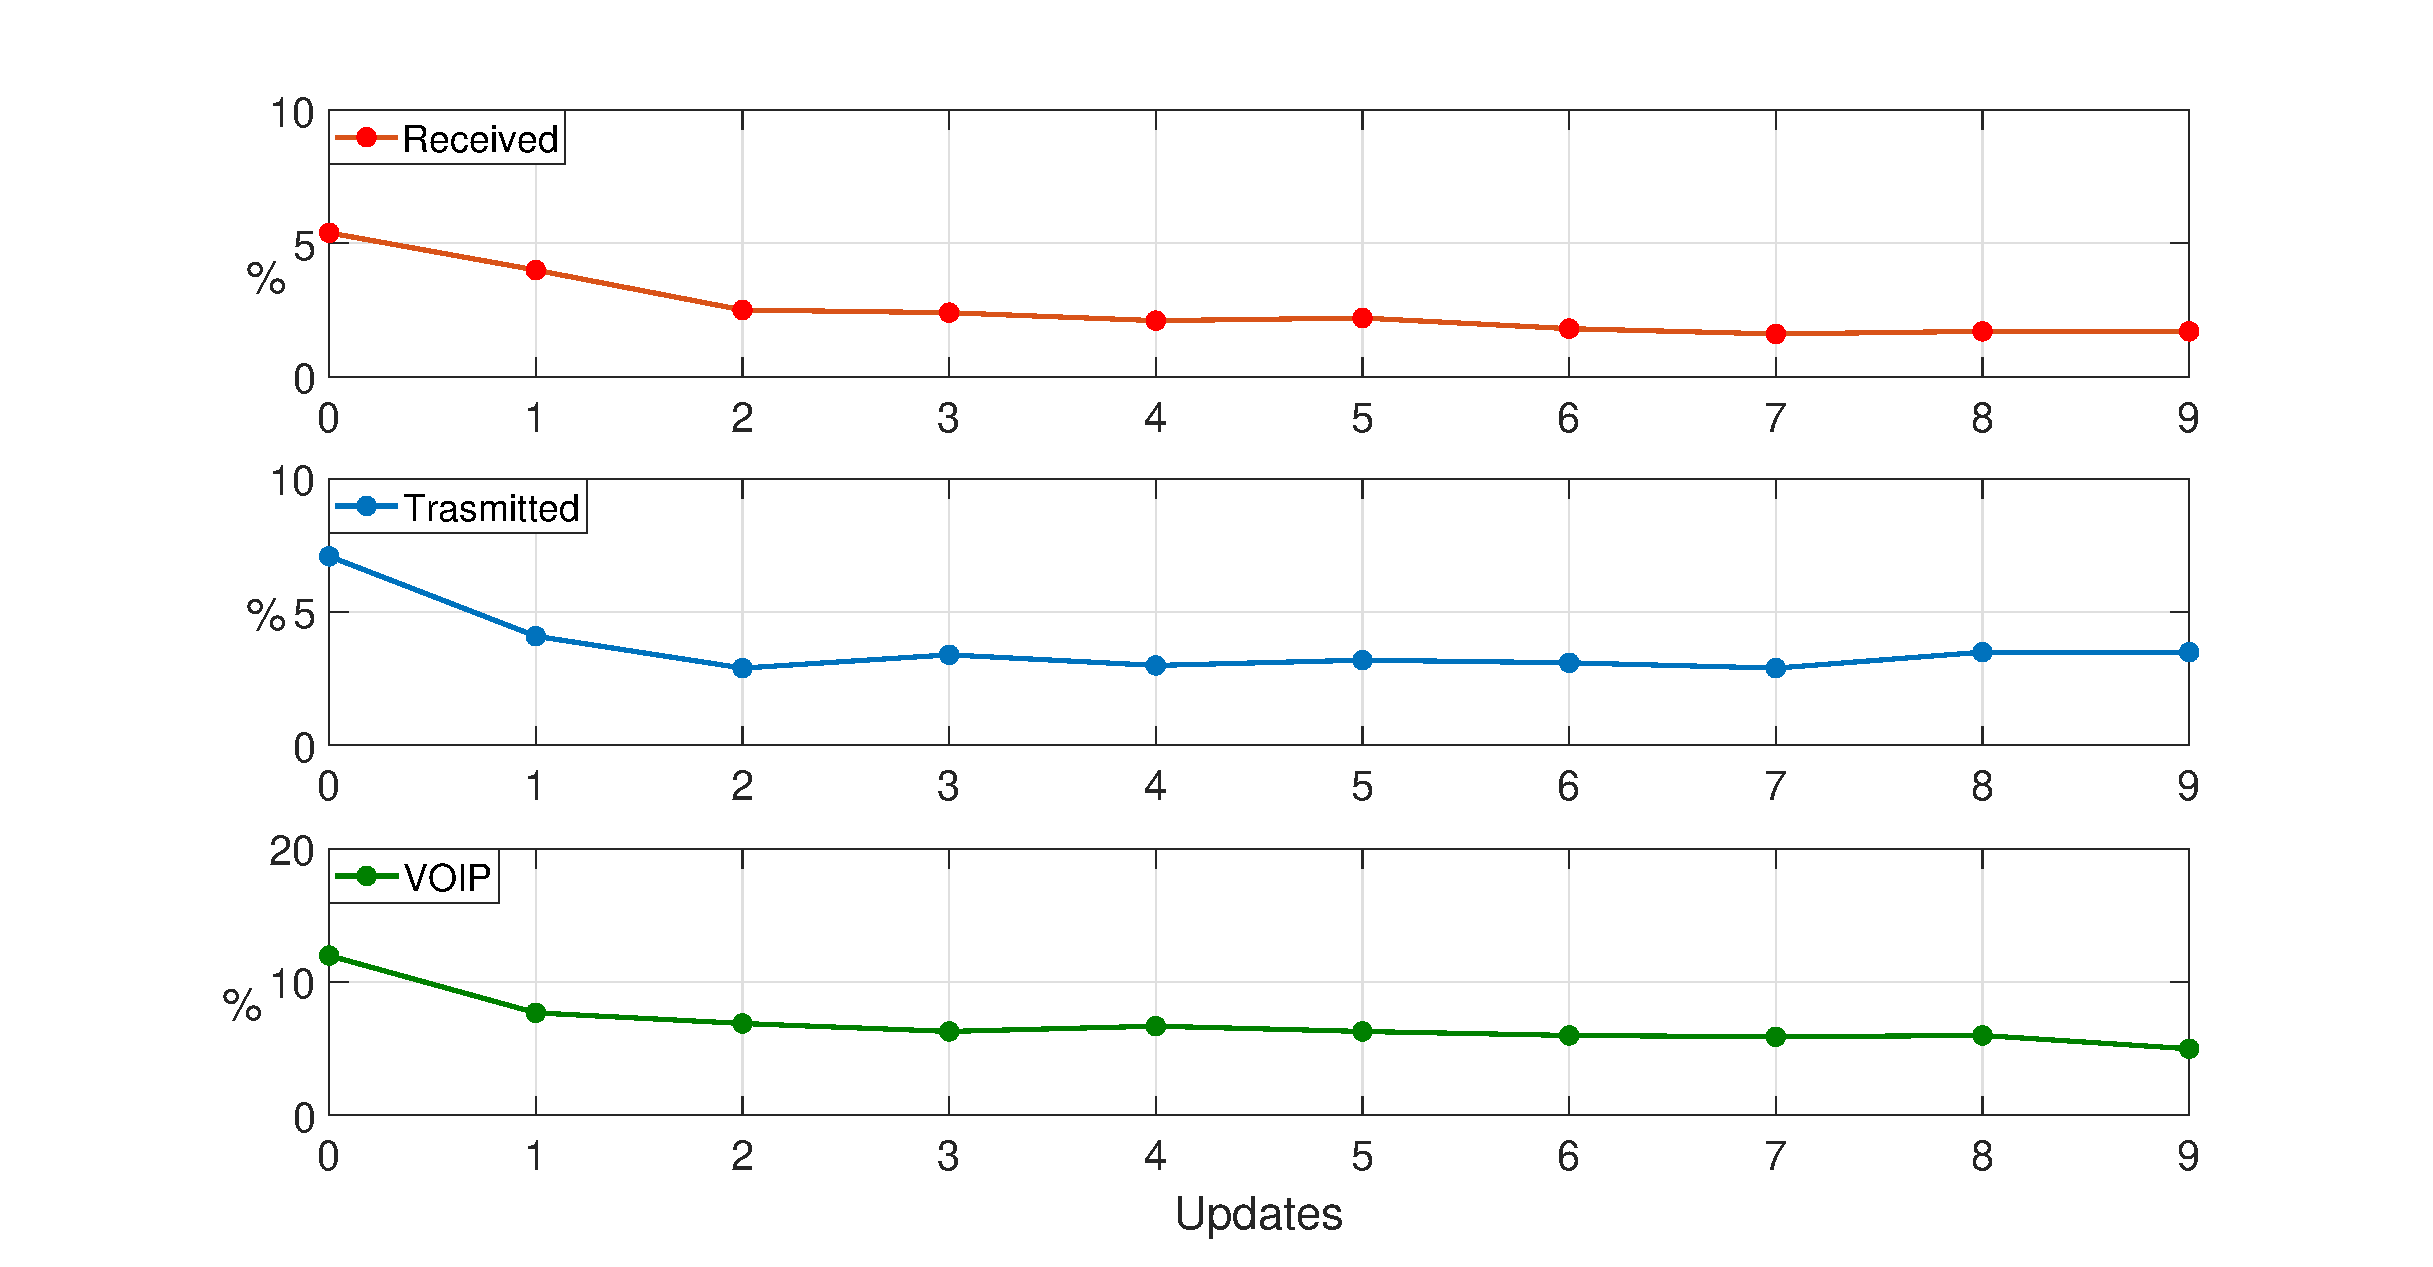
\includegraphics[trim={120 0 120 0}, width=1\linewidth]{figure/NEWSETUP_PESCARA.eps}
	\caption{NRMSE of the packets predictive model at prediction horizon of N=1 with different updated models. Every update add 288 samples (about 1 day) to the previous model training data.}
	\label{fig:{NEWSETUP_Pescara}}
\end{figure}